
\subsection{Recipes for engineering templates}
\label{ssec:recipes_technical}

% HB 20230726: We decided that the recipes listed here should be included.
%\TBD It is not clear (2020-11-19) whether data from maintenance
%templates need to be reduced by the pipeline. This section and the
%recipes described therein serves as a placeholder and may be removed
%later.

The CLC coronagraph was removed from the baseline coronagraphic modes before FDR however the coronagraph would be technically available during engineering. At this stage the DRL will not have the corresponding recipes to use the CLC. However, if the need arises during commissioning or after to make the CLC mode available, its DRL recipe can be adapted from the baseline RAVC/CVC coronagraph recipes as it is related in design and usage.

%------------------------------------------------------------------------------------------------------------------
\subsubsection{\REC*{metis_pupil_imaging}: Pupil imaging}\label{rec:metis_pupil_imaging}
\label{sssec:pupil_imaging}

This recipe refers to pupil imaging using the science detectors.
Pupil imaging is needed to verify the alignment and illumination of the pupil masks (part of the HCI coronagraphs) with the telescope beam.
It is not foreseen to be used by scientists in regular operation.

% From OC:
%Presumably it only contains the most basic reduction  steps.
%There may have to be separate recipes for the various
%subsystems.

% From GO:
%Also it can be used to record the pupil transmission which can improve PSF modelling.
%A simple reduction to get rid of bias effects might be enough to align the pupil, and it might already be possible on the raw data.
%If they want pupil transmission they likely also expect some pixel response or flatfield correction.

\begin{recipedef}
  Name                 & \REC{metis_pupil_imaging}                     \\
  Purpose:             & Apply basic reduction to pupil imaging data.  \\
  Requirements:        & --                                            \\
  Type:                & Maintenance                                   \\
  Templates:           & \TPL{METIS_pup_lm}                            \\
                       & \TPL{METIS_pup_n}                             \\
  Input data:          & \RAW{LM_PUPIL_RAW} or \RAW{N_PUPIL_RAW}       \\
                       & \STATCALIB{GAIN_MAP_2RG} or \STATCALIB{GAIN_MAP_GEO}    \\
  Matched keywords:    & \FITS{DRS.PUPIL}                              \\
  Algorithm            & Apply dark current and flat field corrections.\\
  Output data:         & \PROD{LM_PUPIL_REDUCED} or \PROD{N_PUPIL_REDUCED} \\
  Expected accuracies: & n/a                                           \\
  QC1 parameters:      & None                                          \\
\end{recipedef}

\clearpage
%------------------------------------------------------------------------------------------------------------------
\clearpage
\subsubsection{\REC*{metis_cal_chophome}: Chopper home position recipe}
\label{sssec:metiscalchophome}
\label{sssec:metis_cal_chophome}
\label{metis_cal_chophome}
\label{rec:metiscalchophome}
\label{rec:metis_cal_chophome}

The recipe \REC{metis_cal_chophome} aims to detect chopper mirror zero positions. It is foreseen to be carried out on a daily basis; at the very least it is necessary after changes that possibly affect the absolute chopper position, e.g.\ after instrument interventions or unforeseen events like earthquakes (cf.\ Section ``Chopper Home Position'' in  \cite{METIS-calibration_plan}).

The procedure consists in measuring the position of a point source
from the \ac{WCU}, which has been centred on the \ac{WFS} pyramid (in
the K-band), in the \CODE{IMG_LM} mode.  The recipe measures the
position of the point source on the LM detector and derives a
coordinate offset between the \ac{WFS} Pyramid focal plane and the
science focal planes by comparing to the respective positional
metrology values of the \ac{WFS} field selector and the chopper.
%  (the latter in plural because we have already calibrated the relative astrometry between between IMG-LM and IMG-N/LMS).

\begin{recipedef}
Name:		& \REC{metis_cal_chophome} \\
Purpose:	& Detection of the chopper mirror home position \\
Type:		& Calibration\\
Requirements: & None \\
Templates:      & \TPL{METIS_img_lm_cal_ChopperHome} \\
Input data:     & \RAW{LM_CHOPHOME_RAW} \\
                & \RAW{LM_WCU_OFF_RAW} \\
                & \EXTCALIB{PERSISTENCE_MAP}  \\
                & \STATCALIB{LINEARITY_2RG}  \\
                & \STATCALIB{GAIN_MAP_2RG}  \\
                & \EXTCALIB{BADPIX_MAP_2RG}  \\
Matched Keywords & \FITS{DET.DIT} \\
                 & \FITS{DET.NDIT} \\
                 & \FITS{DRS.FILTER} \\
Parameters: 	& None\\
Algorithm:      & remove detector signature\\
                & remove median background\\
                & detect reference source from \ac{WCU} via centroid peak detection\\
                & Calculate mirror offset\\
Output data:	& Stacked chopperhome image \\
                & Offset of the chopper mirror (as header keywords) to be piped either into the \ac{ICS} for correction  or to be used in the pipeline for astrometric correction\\
Expected accuracies: & 0.1\,mas accuracy of the centroid position (cf.~\cite{METIS-calibration_plan})\\
QC1 parameters: & \QC{QC CAL CHOPHOME XCEN} \\
                & \QC{QC CAL CHOPHOME XCEN STDEV} \\
                & \QC{QC CAL CHOPHOME YCEN} \\
                & \QC{QC CAL CHOPHOME YCEN STDEV} \\
                & \QC{QC CAL CHOPHOME FWHM} \\
                & \QC{QC CAL CHOPHOME SNR} \\
                & \QC{QC CAL CHOPHOME OFFX} \\
                & \QC{QC CAL CHOPHOME OFFY} \\

\end{recipedef}


\begin{figure}[hb]
  \centering
  \def \globalscale {0.600000}
  \fontsize{10}{12}\selectfont
  
% ADDING NEW DEFINITIONS -------------------------------------------- start
\definecolor{listingbg}{gray}{0.95}
\definecolor{darkgreen}{rgb}{0.0, 0.7, 0.0}
\definecolor{darkblue} {rgb}{0.0, 0.0, 0.7}
\definecolor{cyan} {rgb}{0.0, 0.4, 0.4}
\definecolor{darkred}  {rgb}{0.7, 0.0, 0.0}
\definecolor{darkorange}{rgb}{1.0, 0.49, 0.0}
\definecolor{violett}{rgb}{255, 0, 255}
\definecolor{turq}{rgb}{0.0, 0.7, 0.8}
\definecolor{fits}{rgb}{0.4, 0.1, 1}


\makeatletter
\lstdefinestyle{RAWstyle}{%
  basicstyle=\ttfamily\color{black}%
  \lst@ifdisplaystyle\scriptsize\fi}

\lstdefinestyle{PARstyle}{%
  basicstyle=\ttfamily\color{black}%
  \lst@ifdisplaystyle\scriptsize\fi}

\lstdefinestyle{DRLstyle}{%
  basicstyle=\ttfamily\color{black}%
  \lst@ifdisplaystyle\scriptsize\fi}

\lstdefinestyle{RECstyle}{%
  basicstyle=\ttfamily\color{black}%
  \lst@ifdisplaystyle\scriptsize\fi}

\lstdefinestyle{QCstyle}{%
  basicstyle=\ttfamily\color{black}%
  \lst@ifdisplaystyle\scriptsize\fi}

\lstdefinestyle{TPLstyle}{%
  basicstyle=\ttfamily\color{black}%
  \lst@ifdisplaystyle\scriptsize\fi}

\lstdefinestyle{PRODstyle}{%
  basicstyle=\ttfamily\color{black}%
  \lst@ifdisplaystyle\scriptsize\fi}

\lstdefinestyle{EXTCALIBstyle}{%
  basicstyle=\ttfamily\color{black}%
  \lst@ifdisplaystyle\scriptsize\fi}

\lstdefinestyle{STATCALIBstyle}{%
  basicstyle=\ttfamily\color{black}%
  \lst@ifdisplaystyle\scriptsize\fi}
\makeatother

%%% This file contains definitions of shapes and nodes used
%%% for a recipe workflow
%%% Author       : Oliver Czoske
%%% Created      : 2021-03-03
%%% Last Changed : 2021-03-03
%%% Changes:
%%%

\usetikzlibrary{
  shapes.misc,
  positioning,
  calc,
  arrows.meta}

%% All connecting lines have an arrow
\tikzset{
  connection_arrow/.style={->, >=Latex[open], thick}
}

%% Start and stop buttons (black disks, stop with ring)
%% These are pics, use as
%%         \pic (name) [above of=..] {picname};
\tikzset{
  start/.pic = {
    \node (-m) at (0, 0){};
    \filldraw [fill=black] (0, 0) circle (0.2);
  }
}

\tikzset{
  stop/.pic = {
    \node (-m) at (0, 0){};
    \node (-t) at (0, -0.3){};
    \filldraw [fill=black] (0, 0) circle(0.2);
    \draw[black] (0, 0) circle (0.3);
  }
}


%%%% Various boxes and their colours
%%%% These are nodes, use as
%%%% \node (name) [type, location]  {text};

\definecolor{stepcolor}{RGB}{210,169,188}
\definecolor{rawcolor}{RGB}{205,205,205}
\definecolor{externalcolor}{RGB}{183,255,255}
\definecolor{calibcolor}{RGB}{255,250,216}
\definecolor{calproductcolor}{RGB}{185,184,237}
\definecolor{qcproductcolor}{RGB}{255,201,165}
\definecolor{sciproductcolor}{RGB}{197,219,183}
\definecolor{framecolor}{RGB}{127,13,65}

\tikzset{
  %% template : the template(s) that trigger(s) the recipe
  template/.style={
    rectangle,
    draw=black,
    minimum width=4.0cm,
    minimum height=0.5cm,
    align=center
  },
  %% input : the input files
  input/.style={
    rectangle,
    fill=rawcolor,
    minimum width=4.0cm,
    minimum height=0.75cm,
%     text width=3cm,
    align=center
  },
  %% calib : calibration input
  calib/.style={
    rectangle,
    fill=calibcolor,
    minimum width=4.0cm,
    minimum height=0.75cm,
%     text width=3cm,
    align=center
  },
  %% external : external input
  external/.style={
    rectangle,
    fill=externalcolor,
    minimum width=4.0cm,
    minimum height=0.75cm,
%     text width=3.5cm,
    align=center
  },
  %% params : parameters
  params/.style={
    rectangle,
    draw=red,
    thick,
    minimum width=4.0cm,
    minimum height=0.75cm,
%     text width=3cm,
    align=center
  },
  %% redstep : a reduction step
  %%      ("step" is predefined and can't be used)
  redstep/.style={
    rectangle,
    rounded corners=0.2cm,
    fill=stepcolor,   %%% define colour!
    minimum width=4.0cm,
    minimum height=1cm,
%     text width=3cm,
    align=center
  },
  %% connection : connection to input or output
  connection/.style={
    circle,
    fill=black,
    minimum size=0.15cm,
    inner sep=0pt
  },
  %% sciproduct : a science product
  sciproduct/.style={
    rectangle,
    fill=sciproductcolor,
    minimum width=4.0cm,
    minimum height=0.75cm,
%     text width=3.5cm,
    align=center
  },
  %% calproduct : a calibration product
  calproduct/.style={
    rectangle,
    fill=calproductcolor,
    minimum width=4.0cm,
    minimum height=0.75cm,
%     text width=3.5cm,
    align=center
  },
  %% frame : frame around the recipe
  %% This is a path, use as
  %%    \draw [frame] (upper left) rectangle (lower right);
  frame/.style={framecolor, very thick, dashed}
}


\begin{tikzpicture}
  [x=1cm,
  y=-1cm,
  align=center,
  node distance=2cm and 3cm]
  \sffamily

  %% Grid for orientation. Comment out for final figure!
  % \draw[help lines, green](-5, 0) grid (8, 11);

  %%% Put workflow commands here:
  %% Main reduction workflow

  %% template names
  \node (template) [template] {\TPL{METIS_img_lm_cal_ChopperHome}};

  \pic (start)[below=0.75cm of template]{start};

  \node (input) [below=0.75cm of start-m, input] {%
    \textsl{N$_{\mathsf{on}}$} \RAW{LM_CHOPHOME_RAW}\\
    \textsl{N$_{\mathsf{off}}$} \RAW{LM_WCU_OFF_RAW}
  };

  \node (step_signature) [below=4.0cm of input, redstep]{%
    detector signature\\ removal};

  \node (step_subtract) [below=1.cm of step_signature, redstep]{%
    median-combine WCU\_OFF\\ subtract from CHOPHOME};

  \node (step_locate) [below=1.5cm of step_subtract, redstep]{%
    Centroid peak\\ detection};

  \node (step_fit) [below=1.cm of step_locate, redstep]{%
    offset calculation};

  \pic (stop) [below=1.5cm of step_fit]{stop};

  %% Input
  \node (connect_bpm) [connection] at ($(input)!0.3!(step_signature)$) {};
  \node (bpm) [left=3.75cm of connect_bpm, external] {\EXTCALIB{BADPIX_MAP_2RG}};
  \draw [connection_arrow, dashed] (bpm) -- (connect_bpm);

  \node (connect_gain) [connection] at ($(input)!0.47!(step_signature)$) {};
  \node (gain) [left=3.75cm of connect_gain, external] {\EXTCALIB{GAIN_MAP_2RG}};
  \draw [connection_arrow] (gain) -- (connect_gain);

  \node (connect_linearity) [connection] at ($(input)!0.64!(step_signature)$){};
  \node (linearity) [left=3.75cm of connect_linearity, external]{\EXTCALIB{LINEARITY_2RG}};
  \draw [connection_arrow] (linearity) -- (connect_linearity);

  \node (connect_persistence) [connection] at ($(input)!0.81!(step_signature)$){};
  \node (persistence) [left=3.75cm of connect_persistence, external]{\EXTCALIB{PERSISTENCE_MAP}};
  \draw [connection_arrow, dashed] (persistence) -- (connect_persistence);

%  \node (connect_bpmin) [connection] at ($(step_subtract)!0.3!(step_locate)$) {};
%  \node (bpmin) [left=of connect_bpmin, calproduct] {\STATCALIB{BADPIX_MAP_2RG}};
%  \draw [connection_arrow] (bpmin) -- (connect_bpmin);

  \node (connect_background) [connection] at
  ($(step_subtract)!0.35!(step_locate)$) {};
  \node (background) [right=3.5cm of connect_background, calproduct,
                      minimum width=4cm]{%
    \PROD{LM_CHOPHOME_BACKGROUND}};
  \draw [connection_arrow, dashed] (connect_background) -- (background);

  \node (connect_pinhole) [connection] at
  ($(step_subtract)!0.55!(step_locate)$) {};
  \node (pinhole) [left=3.75cm of connect_pinhole, external] {\EXTCALIB{PINHOLE_TABLE}};
  \draw [connection_arrow] (pinhole) -- (connect_pinhole);

  %% Connections
  \draw [connection_arrow] (start-m) -- (input);
  \draw [connection_arrow] (input) -- (step_signature);
  \draw [connection_arrow] (step_signature) -- (step_subtract);
  \draw [connection_arrow] (step_subtract) -- (step_locate);
  \draw [connection_arrow] (step_locate) -- (step_fit);
  \draw [connection_arrow] (step_fit) -- (stop-t);

  %% Output
  \node (connectoutput) [connection] at
  ($(step_fit)!0.5!(stop-t)$) {};
  \node (output) [right=3.5cm of connectoutput, calproduct, minimum width=4cm]{%
    \PROD{LM_CHOPHOME_COMBINED}};
  \draw [connection_arrow] (connectoutput) -- (output);

  %% Frame around recipe
  \draw [frame]
  ($(input)!0.15!(step_subtract) - (3.5,0)$) rectangle
  ($(step_fit)!0.65!(stop-t) + (3.05,0)$);
  \node [framecolor, anchor=south west] at
  ($(input)!0.16!(step_subtract) - (3.5, 0)$){%
    \REC{metis_cal_chophome}};

\end{tikzpicture}

% ADDING NEW DEFINITIONS -------------------------------------------- start
\definecolor{listingbg}{gray}{0.95}
\definecolor{darkgreen}{rgb}{0.0, 0.7, 0.0}
\definecolor{darkblue} {rgb}{0.0, 0.0, 0.7}
\definecolor{cyan} {rgb}{0.0, 0.4, 0.4}
\definecolor{darkred}  {rgb}{0.7, 0.0, 0.0}
\definecolor{darkorange}{rgb}{1.0, 0.49, 0.0}
\definecolor{violet}{rgb}{255, 0, 255}
\definecolor{turq}{rgb}{0.0, 0.7, 0.8}
\definecolor{fits}{rgb}{0.4, 0.1, 1}


\makeatletter
\lstdefinestyle{RAWstyle}{%
  basicstyle=\ttfamily\color{fits}%
  \lst@ifdisplaystyle\scriptsize\fi}

\lstdefinestyle{PARstyle}{%
  basicstyle=\ttfamily\color{cyan}%
  \lst@ifdisplaystyle\scriptsize\fi}

\lstdefinestyle{DRLstyle}{%
  basicstyle=\ttfamily\color{violet}%
  \lst@ifdisplaystyle\scriptsize\fi}

\lstdefinestyle{RECstyle}{%
  basicstyle=\ttfamily\color{darkgreen}%
  \lst@ifdisplaystyle\scriptsize\fi}

%% Write QC parameters like this: \QC{QC_SOMETHING_OR_OTHER}
\lstdefinestyle{QCstyle}{%
  basicstyle=\ttfamily\color{darkblue}%
  \lst@ifdisplaystyle\scriptsize\fi}

%% Write templates like this: \TPL{DARK_LM}
\lstdefinestyle{TPLstyle}{%
  basicstyle=\ttfamily\color{darkred}%
  \lst@ifdisplaystyle\scriptsize\fi}

%% Write products like this: \hyperref[dataitem:some_thing]{\PROD{SOME_THING}}
\lstdefinestyle{PRODstyle}{%
  basicstyle=\ttfamily\color{darkorange}%
  \lst@ifdisplaystyle\scriptsize\fi}

%% external calib files
\lstdefinestyle{EXTCALIBstyle}{%
  basicstyle=\ttfamily\color{Turquoise}%
  \lst@ifdisplaystyle\scriptsize\fi}

% static calib files
\lstdefinestyle{STATCALIBstyle}{%
  basicstyle=\ttfamily\color{teal}%
  \lst@ifdisplaystyle\scriptsize\fi}
\makeatother


%%% Local Variables:
%%% mode: latex
%%% TeX-master: "all"
%%% End:

  \caption[Recipe: \REC*{metis_cal_chophome}]{\REC*{metis_cal_chophome} --
    measurement of the zero position of the chopper mirror.}
  \label{fig:metis_cal_chophome}
\end{figure}

\clearpage

%------------------------------------------------------------------------------------------------------------------
% Moved to https://github.com/AstarVienna/METIS_DRLD/issues/101
% \subsubsection{Plate-scale calibration}
% \TODO{Plate-scale calibration}

%------------------------------------------------------------------------------------------------------------------
\clearpage
\subsubsection{\REC*{metis_lm_adc_slitloss} and \REC*{metis_n_adc_slitloss}: Slit loss determination }\label{sssec:adc_slitlosses}
The recipes \REC{metis_lm_adc_slitloss} (Fig.~\ref{Fig:rec_lm_adc_slitloss}) and \REC{metis_n_adc_slitloss} (Fig.~\ref{Fig:rec_n_adc_slitloss}) aims to determine the throughput as function of the object position along the across-slit direction. It is expected that the usage of the fixed positioned \ac{ADC} will introduce flux losses (cf. Section "Calibration of slit losses" in  \cite{METIS-calibration_plan}). For the determination, the point sources (i.e. mask of the \ac{WCU}) is placed on several positions (distance $\sim\frac{1}{10}\lambda/D$) across the slit (cf. Fig.~\ref{Fig:slitloss}), and measure the wavelength dependent flux changes with respect to the respective positions. Finally, a simple model is determined to be able to correct for the flux losses  (see Section "Calibration of slit losses" in the Calibration Plan~\cite{METIS-calibration_plan} for more details). This recipe is to be carried out once in a while to update the static calibration database.
\begin{figure}[ht]
  \centering
  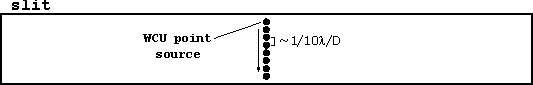
\includegraphics[width=0.5\textheight]{figures/slitloss_det.pdf}
  \caption[slitloss determination]{Algorithm for the slit-loss determination in recipe \REC{metis_lm_adc_slitloss} }
  \label{Fig:slitloss}
\end{figure}

\begin{figure}[ht]
  \centering
  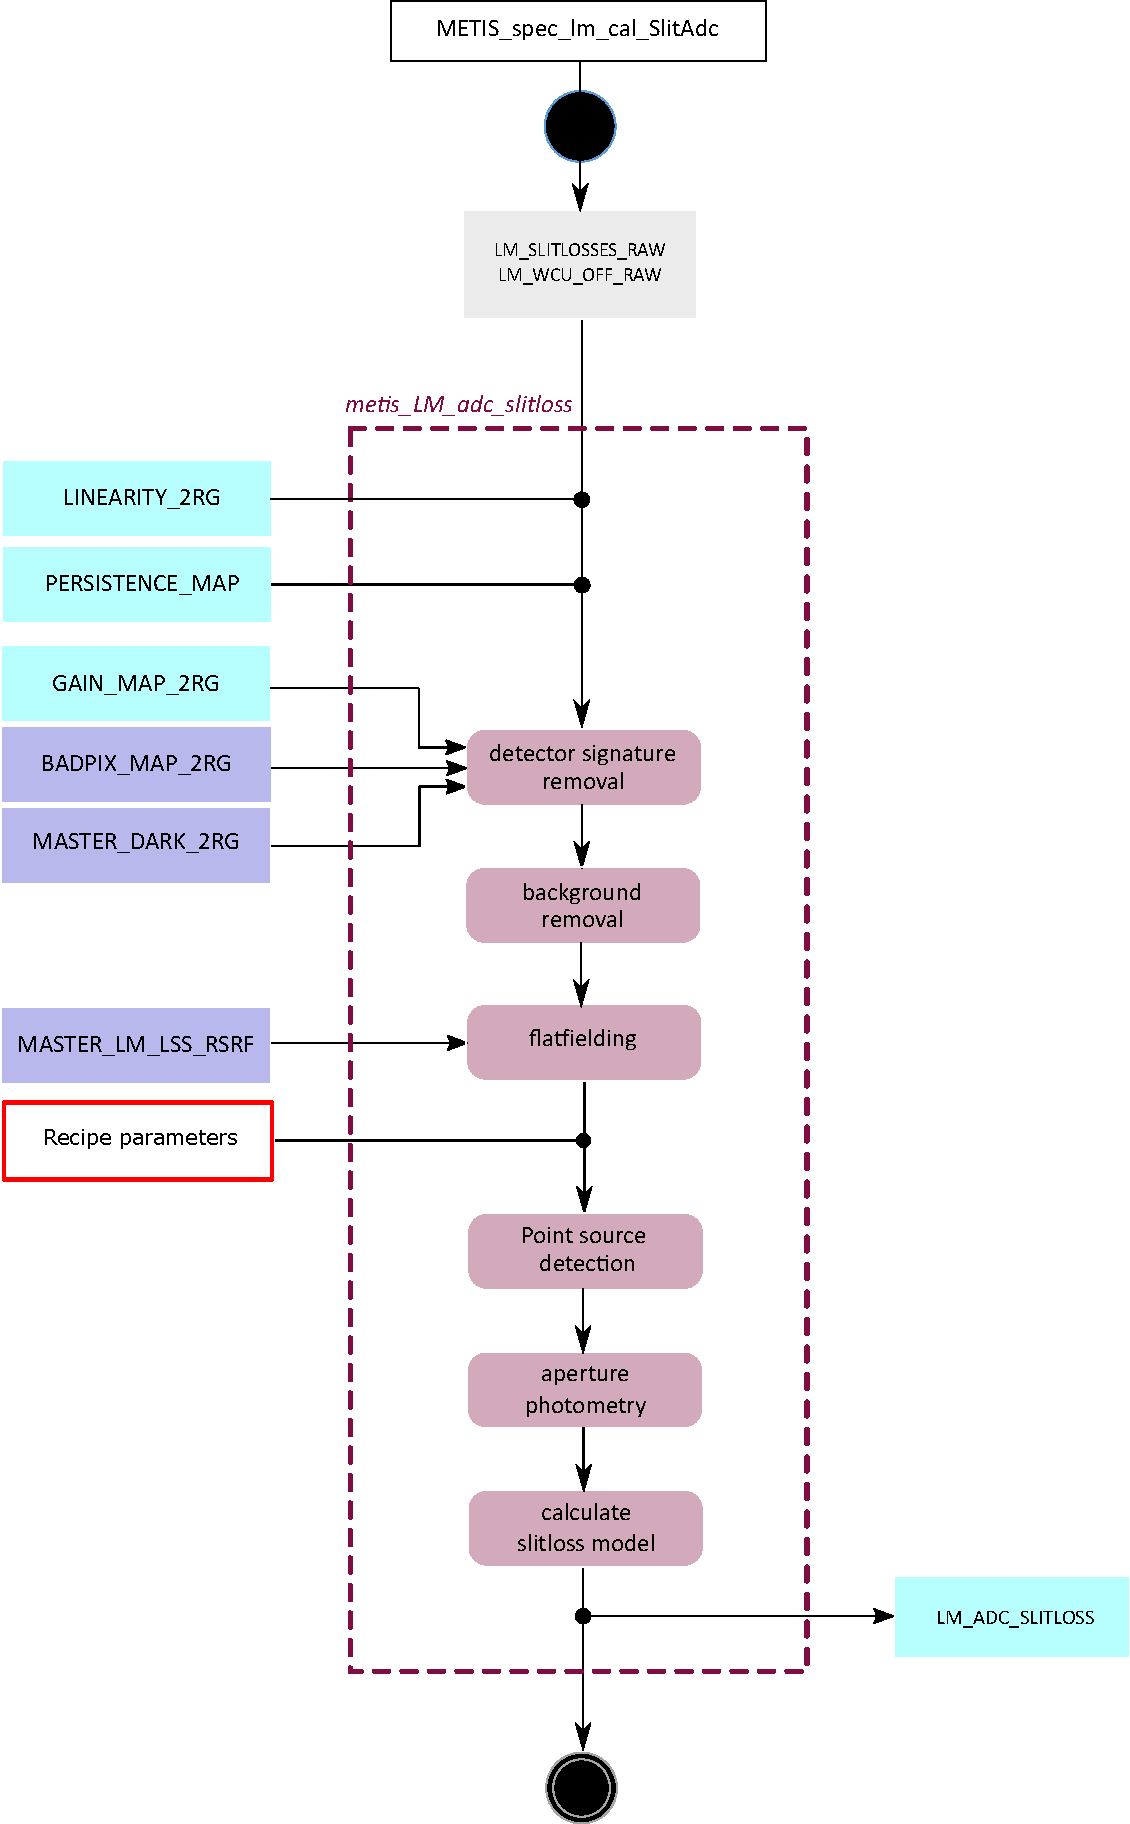
\includegraphics[width=0.5\textheight]{figures/metis_lm_adc_slitloss_v0.83.pdf}
  \caption[Recipe: \REC*{metis_lm_adc_slitloss}]{\REC*{metis_lm_adc_slitloss} --
    Recipe workflow to determine the \ac{ADC} induced slit losses.}
  \label{Fig:rec_lm_adc_slitloss}
\end{figure}

\begin{recipedef}\label{rec:metislmadcmslitloss}\label{rec:metis_lm_adc_slitloss}
Name:		& \REC{metis_lm_adc_slitloss} \\
Purpose:	& Determination of the \ac{ADC} induced slit losses \\
Type:		& Calibration\\
Requirements: &  METIS-6074, METIS-2757, METIS-9099, METIS-9150\\
Templates:           & \TPL{METIS_spec_lm_cal_SlitAdc} \\
Input data:     & \RAW{LM_SLITLOSSES_RAW} \\
                & \RAW{LM_WCU_OFF_RAW} \\
                & \EXTCALIB{PERSISTENCE_MAP}  \\
                & \STATCALIB{LINEARITY_2RG}  \\
                & \STATCALIB{GAIN_MAP_2RG}  \\
                & \EXTCALIB{BADPIX_MAP_2RG}  \\
                & \PROD{MASTER_DARK_2RG}  \\
                & \PROD{MASTER_IMG_FLAT_LAMP_LM}  \\
Matched Keywords & \FITS{DET.DIT} \\
                 & \FITS{DET.NDIT} \\
                 & \FITS{DRS.FILTER} \\
Parameters: 	& exposure time, offset positions\\
Algorithm:      & remove detector signature\\
                & remove dark\\
                & apply flatfield\\
                & detect reference source from \ac{WCU} via centroid peak detection\\
                & apply aperture photometry\\
                & calculate (simple) slitloss model (details to be defined)\\
Output data:	& \STATCALIB{LM_ADC_SLITLOSS} (Slit loss model as function of the wavelength and object position across the slit \\
Expected accuracies: & 3\% (cf.~\cite{METIS_calerrbudget})\\
%QC1 parameters: & \QC{TBD}: TBD\\
\end{recipedef}


\begin{figure}[ht]
  \centering
  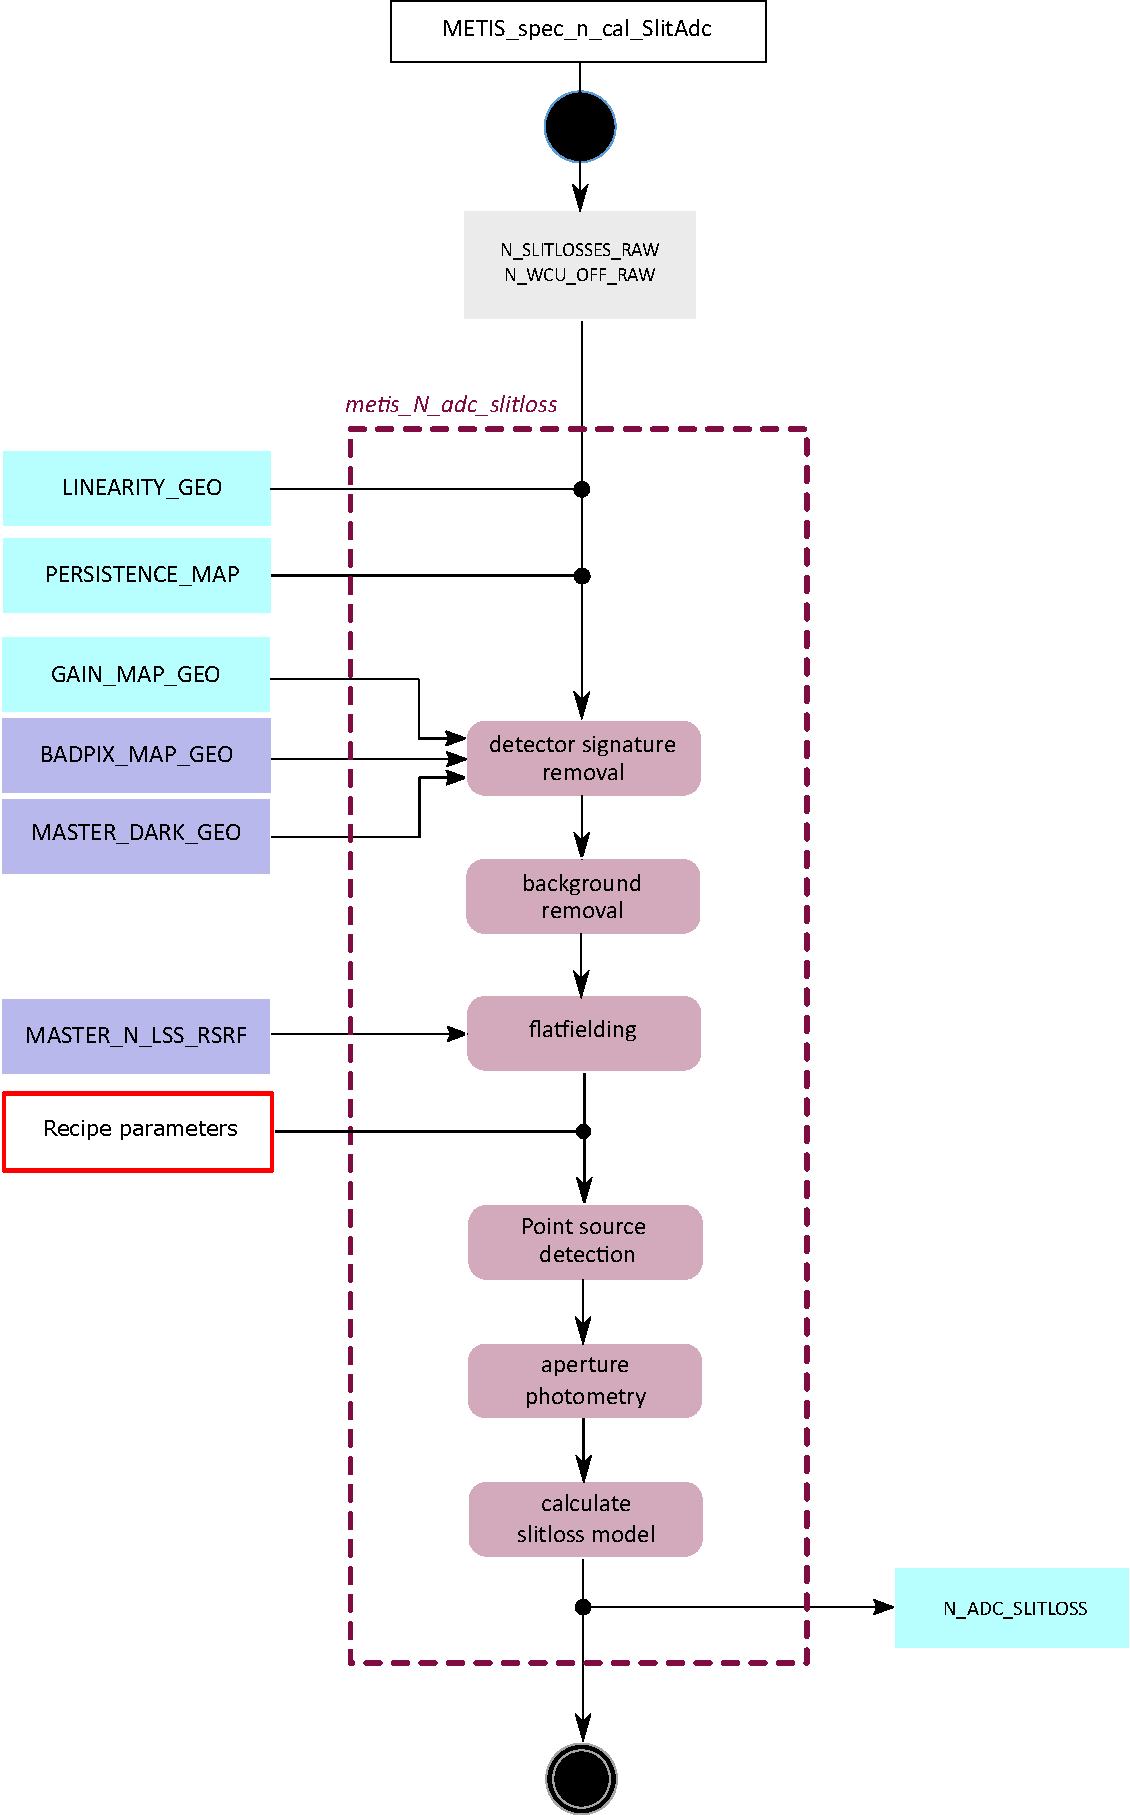
\includegraphics[width=0.5\textheight]{figures/metis_n_adc_slitloss_v0.83.pdf}
  \caption[Recipe: \REC*{metis_n_adc_slitloss}]{\REC*{metis_n_adc_slitloss} --
    Recipe workflow to determine the \ac{ADC} induced slit losses.}
  \label{Fig:rec_n_adc_slitloss}
\end{figure}

\begin{recipedef}\label{rec:metisnadcmslitloss}\label{rec:metis_n_adc_slitloss}
Name:		& \REC{metis_n_adc_slitloss} \\
Purpose:	& Determination of the \ac{ADC} induced slit losses \\
Type:		& Calibration\\
Requirements: & METIS-6074, METIS-2757, METIS-9099, METIS-9150 \\
Input data:     & \RAW{N_SLITLOSSES_RAW} \\
                & \RAW{N_WCU_OFF_RAW} \\
                & \EXTCALIB{PERSISTENCE_MAP}  \\
                & \STATCALIB{LINEARITY_GEO}  \\
                & \STATCALIB{GAIN_MAP_GEO}  \\
                & \EXTCALIB{BADPIX_MAP_GEO}  \\
                & \PROD{MASTER_DARK_GEO}  \\
& \PROD{MASTER_IMG_FLAT_LAMP_N}  \\
Matched Keywords & \FITS{DET.DIT} \\
                 & \FITS{DET.NDIT} \\
                 & \FITS{DRS.FILTER} \\
Parameters: 	& exposure time, offset positions\\
Algorithm:      & remove detector signature\\
                & remove dark\\
                & apply flatfield\\
                & detect reference source from \ac{WCU} via centroid peak detection\\
                & apply aperture photometry\\
                & calculate (simple) slitloss model (details to be defined)\\
Output data:	& \STATCALIB{N_ADC_SLITLOSS} (Slit loss model as function of the wavelength and object position across the slit) \\
Expected accuracies: & 3\% (cf.~\cite{METIS_calerrbudget})\\\\
%QC1 parameters: & \QC{TBD}: TBD\\
\end{recipedef}

%------------------------------------------------------------------------------------------------------------------
\subsubsection{Fringing correction}
\label{rec:metis_fringing_correction}

It is unclear for the time being how much of a problem will be with the METIS
detectors, and what the best strategy will be to tackle it. Therefore, the
method to use will be chosen based on AIT results (\REQ{METIS-9151}, for rationale and basic method description see Ch.~3.12 in the Calibration Plan~\cite{METIS-calibration_plan}).

Whether a stand-alone recipe will be required, or if the fringe-map will become
part of another recipe, is part of that uncertainty. If needed, the design of
said recipe will be minimal work and is thus omitted in this document.

%%% Local Variables:
%%% mode: latex
%%% TeX-master: "METIS_DRLD"
%%% End:
